\documentclass[unicode,11pt,a4paper,oneside,numbers=endperiod,openany]{scrartcl}
\usepackage{amsmath}
\usepackage{listings}
\usepackage{enumitem}

\newcommand{\norm}[1]{\lvert\lvert #1 \rvert\rvert}

\renewcommand{\thesubsection}{\arabic{subsection}}

\usepackage{ifthen}
\usepackage[utf8]{inputenc}
\usepackage{graphics}
\usepackage{graphicx}
\usepackage{hyperref}

\pagestyle{plain}
\voffset -5mm
\oddsidemargin  0mm
\evensidemargin -11mm
\marginparwidth 2cm
\marginparsep 0pt
\topmargin 0mm
\headheight 0pt
\headsep 0pt
\topskip 0pt        
\textheight 255mm
\textwidth 165mm

\newcommand{\duedate} {}
\newcommand{\setduedate}[1]{%
\renewcommand\duedate {\textbf{Due date:}~ #1}}
\newcommand\isassignment {false}
\newcommand{\setassignment}{\renewcommand\isassignment {true}}
\newcommand{\ifassignment}[1]{\ifthenelse{\boolean{\isassignment}}{#1}{}}
\newcommand{\ifnotassignment}[1]{\ifthenelse{\boolean{\isassignment}}{}{#1}}

\newcommand{\assignmentpolicy}{
\begin{table}[h]
\begin{center}
\scalebox{0.8} {%
\begin{tabular}{|p{0.02cm}p{16cm}|}
\hline
&\\
\multicolumn{2}{|c|}{\Large\textbf{Numerical Computing 2023 ---  Submission Instructions}}\\
\multicolumn{2}{|c|}{\large\textbf{(Please, notice that following instructions are mandatory: }}\\
\multicolumn{2}{|c|}{\large\textbf{submissions that don't comply with, won't be considered)}}\\
&\\
\textbullet & Assignments must be submitted to \href{https://www.icorsi.ch/course/view.php?id=14666}{iCorsi} (i.e. in electronic format).\\
\textbullet & Provide both executable package and sources (e.g. C/C++ files, MATLAB). 
If you are using libraries, please add them in the file. Sources must be organized in directories called:\\
\multicolumn{2}{|c|}{\textit{Project\_number\_lastname\_firstname}}\\
& and  the  file must be called:\\
\multicolumn{2}{|c|}{\textit{project\_number\_lastname\_firstname.zip}}\\
\multicolumn{2}{|c|}{\textit{project\_number\_lastname\_firstname.pdf}}\\
\textbullet &  The TAs will grade your project by reviewing your project write-up, and looking at the implementation you attempted, and benchmarking your code's performance.\\

\textbullet & You are allowed to discuss all questions with anyone you like; however: (i) your submission must list anyone you discussed problems with and (ii) you must write up your submission independently.\\
\hline
\end{tabular}
}
\end{center}
\end{table}
}
\newcommand{\punkte}[1]{\hspace{1ex}\emph{\mdseries\hfill(#1~\ifcase#1{Points}\or{Points}\else{Points}\fi)}}


\newcommand\serieheader[6]{
\thispagestyle{empty}%
\begin{flushleft}

\includegraphics[width=0.45\textwidth]{CI_logo}
\end{flushleft}
  \noindent%
  {\large\ignorespaces{\textbf{#1}}\hspace{\fill}\ignorespaces{ \textbf{#2}}}\\ \\%
  {\large\ignorespaces #3 \hspace{\fill}\ignorespaces #4}\\
  \noindent%
  \bigskip
  \hrule\par\bigskip\noindent%
  \bigskip {\ignorespaces {\Large{\textbf{#5}}}
  \hspace{\fill}\ignorespaces \large \ifthenelse{\boolean{\isassignment}}{\duedate}{#6}}
  \hrule\par\bigskip\noindent%  \linebreak
 }

\makeatletter
\def\enumerateMod{\ifnum \@enumdepth >3 \@toodeep\else
      \advance\@enumdepth \@ne
      \edef\@enumctr{enum\romannumeral\the\@enumdepth}\list
      {\csname label\@enumctr\endcsname}{\usecounter
        {\@enumctr}%%%? the following differs from "enumerate"
	\topsep0pt%
	\partopsep0pt%
	\itemsep0pt%
	\def\makelabel##1{\hss\llap{##1}}}\fi}
\let\endenumerateMod =\endlist
\makeatother




\usepackage{textcomp}





\begin{document}


\setassignment
\setduedate{Wednesday, 22 November 2023, 11:59 PM}

\serieheader{Numerical Computing}{2023}{\textbf{Student:} Hun Rim}{\textbf{Discussed with:} Georgy Batyrev}{Bonus assignment}{}
\newline

\assignmentpolicy


\newpage

\section*{Exercise 1: Inconsistent systems of equations [10 points]}
Consider the following inconsistent systems of equations: \\

\begin{center}
(a) ${A_1x = b_1}$, where

\vspace{10px}

\begin{equation*}
A_1 =
\begin{bmatrix}
1 & 0 \\
1 & 0 \\
1 & 0
\end{bmatrix}
b_1=
\begin{bmatrix}
5 \\
2 \\
4
\end{bmatrix}
\end{equation*}
\end{center}

\begin{center}
(b) ${A_2x = b_2}$, where

\vspace{10px}

\begin{equation*}
A_2 =
\begin{bmatrix}
1 & 1 & 0 \\
0 & 1 & 1 \\
1 & 2 & 1 \\
1 & 0 & 1
\end{bmatrix}
b_2=
\begin{bmatrix}
2 \\
2 \\
3 \\
4
\end{bmatrix}
\end{equation*}
\end{center}

Find the least squares solution ${x^*}$ and compute the Euclidean norm of the residual, SE and RMSE. \\

\textbf{solution:} \\
Least Square solution ${x^*}$ can be obtained by solving the following equation:

\vspace{20px}

\begin{equation}
 A^TAx = A^Tb
\end{equation}

\vspace{20px}

Then from the ${x^*}$ obtained, we can get the residual vector as following and from it, we can calculate the Euclidean norm and proceed to SE (Standard Error) and RMSE (Root Mean Squared Error):

\vspace{20px}

\begin{equation}
 r = Ax^* - b
\end{equation}

\vspace{20px}

\begin{equation}
 Euclidean Norm = \norm{r}_2
\end{equation}

\vspace{20px}

\begin{equation}
 SE = \norm{r}_2^2
\end{equation}

\vspace{20px}

\begin{equation}
 RMSE = \sqrt{\frac{SE}{m}}
\end{equation}

\vspace{20px}

Where ${m}$ is the number of rows in residual vector. \\

\newpage
(a)
\begin{equation*}
\begin{bmatrix}
1 & 1 & 1 \\
0 & 0 & 0
\end{bmatrix}
\begin{bmatrix}
1 & 0 \\
1 & 0 \\
1 & 0
\end{bmatrix}
x = \begin{bmatrix}
1 & 1 & 1 \\
0 & 0 & 0
\end{bmatrix}
\begin{bmatrix}
5 \\
2 \\
4
\end{bmatrix}
\end{equation*}
\begin{equation*}
 \begin{bmatrix}
  3 & 0 \\
  0 & 0
 \end{bmatrix}x=
 \begin{bmatrix}
  11 \\
  0
 \end{bmatrix}
\end{equation*}
\begin{equation*}
 x^* = \begin{bmatrix}
        3.6667 \\
        0
       \end{bmatrix}
\end{equation*}
\begin{equation*}
 r^* = \begin{bmatrix}
        1 & 0 \\
        1 & 0 \\
        1 & 0
       \end{bmatrix}
       \begin{bmatrix}
        3.6667 \\
        0
       \end{bmatrix} -
       \begin{bmatrix}
        5 \\
        2 \\
        4
       \end{bmatrix} =
       \begin{bmatrix}
        -1.3333\\
        1.6667 \\
        -0.3333
       \end{bmatrix}
\end{equation*}
\begin{equation*}
 EuclideanNorm = \norm{r}_2 = \sqrt{(-1.3333)^2 + (1.6667)^2 + (-0.3333)^2} = \sqrt{4.6667} \approx 2.1602
\end{equation*}

\begin{equation*}
 SE = \norm{r}_2^2 = (-1.3333)^2 + (1.6667)^2 + (-0.3333)^2 \approx 4.6667
\end{equation*}

\begin{equation*}
 RMSE = \sqrt{\frac{\norm{r}_2^2}{m}} \approx \sqrt{\frac{4.6667}{3}} \approx 1.2472 
\end{equation*}

(b)
\begin{equation*}
\begin{bmatrix}
1 & 0 & 1 & 1 \\
1 & 1 & 2 & 0 \\
0 & 1 & 1 & 1
\end{bmatrix}
\begin{bmatrix}
1 & 1 & 0 \\
0 & 1 & 1 \\
1 & 2 & 1 \\
1 & 0 & 1
\end{bmatrix}
x = \begin{bmatrix}
1 & 0 & 1 & 1 \\
1 & 1 & 2 & 0 \\
0 & 1 & 1 & 1
\end{bmatrix}
\begin{bmatrix}
2 \\
2 \\
3 \\
4
\end{bmatrix}
\end{equation*}

\begin{equation*}
 \begin{bmatrix}
  3 & 3 & 2 \\
  3 & 6 & 3 \\
  2 & 3 & 3
 \end{bmatrix}x = 
 \begin{bmatrix}
  9 \\
  10 \\
  9
 \end{bmatrix}
\end{equation*}

If we re-arrange the formula for ${x^*}$ we get:

\begin{equation}
 x^* = (A^T_2A_2)^{-1}A^T_2b_2
\end{equation}

and the resulting ${x^*}$ will be

\begin{equation*}
 x^* \approx \begin{bmatrix}
        2 \\
        -0.3333 \\
        2
       \end{bmatrix}
\end{equation*}

\begin{equation*}
 r = \begin{bmatrix}
1 & 1 & 0 \\
0 & 1 & 1 \\
1 & 2 & 1 \\
1 & 0 & 1
\end{bmatrix}
\begin{bmatrix}
        2 \\
        -0.3333 \\
        2
\end{bmatrix} -
\begin{bmatrix}
2 \\
2 \\
3 \\
4
\end{bmatrix} \approx
\begin{bmatrix}
-0.3333 \\
-0.3333 \\
0.3333 \\
0
\end{bmatrix}
\end{equation*}

\begin{equation*}
 EuclideanNorm = \norm{r}_2 \approx \sqrt{(-0.3333)^2 + (-0.3333)^2 + (0.3333)^2 + (0)^2} \approx \sqrt{0.3333} \approx 0.5774
\end{equation*}

\begin{equation*}
 SE = \norm{r}_2^2 = (-0.3333)^2 + (-0.3333)^2 + (0.3333)^2 + (0)^2 \approx 0.3333
\end{equation*}

\begin{equation*}
 RMSE = \sqrt{\frac{\norm{r}_2^2}{m}} \approx \sqrt{\frac{0.3333}{4}} \approx 0.2887
\end{equation*}

\section*{Exercise 2: Polynomials models for least squares [20 points]}

\begin{enumerate}[label=(\alph*)]
 \item Write ${leastSquare.m}$ function which calculates least squares ${x^*}$, euclidean norm, SE and RMSE of a matrix A and vector b, and write a script ${ex2a.m}$ which computes the result of exercise 1.\\
 
  \begin{lstlisting}[language=Matlab]
  function [x, EuclideanNorm, SE, RMSE] = leastSquares(A, b)
    x = (A' * A) \ A' * b;
    r = A * x - b;
    EuclideanNorm = norm(r);
    SE = EuclideanNorm ^ 2;
    MSE = SE / length(b);
    RMSE = sqrt(MSE);
  end
 \end{lstlisting}
 
 The code above calculates least squares (${leastSquare.m}$) using matlab library function and Euclidean norm is calculated by using the matlab norm function after calculating the residual vector. Standard Errors (SE) are calculated by directly squaring the Euclidean norm, and before the Root Mean Squared Error (RMSE) is calculated, the Mean Squared Error is calculated through dividing SE by length of vector b. \\
 
 \begin{lstlisting}[language=Matlab]
    A_1 = [1, 0; 1, 0; 1, 0];
    b_1 = [5; 2; 4];
    A_2 = [1, 1, 0; 0, 1, 1; 1, 2, 1; 1, 0, 1];
    b_2 = [2; 2; 3; 4];

    [x_1, norm1, SE1, RMSE1] = leastSquares(A_1, b_1);
    [x_2, norm2, SE2, RMSE2] = leastSquares(A_2, b_2);
 \end{lstlisting}
 
 This particular code (${ex2a.m}$) defines the values of matrix A and vector b as given in the exercise 1, and it calculates and stores the least squares, Euclidean Norm, SE, RMSE using function in ${leastSquare.m}$ as described above. Result of the calculation via the script is same as the calculation by hand for (b) of exercise 1, but it differs for the (a). Reason behind this is because script calculation solves for least squares through utilizing inverse like shown in equation 6, whereas when calculating by hand, an algebric approach is taken. As determinant of ${x}$ is equal to 0, script generates ${NaN}$ and Euclidean Norm, SE, RMSE which are calculated from it also generates NaN. However, algebric approach evades this problem, hence, it produces normal result. A solution to this problem would be checking if least squares generated are ${NaN}$ and if true, we use built-in function such as ${pinv(A) * b}$ and otherwise we use the old inverse calculation approach. \\
 
 Debugged code is as following:
 \begin{lstlisting}[language=Matlab]
    determinant = det(A' * A);
    if (determinant == 0)
        x = pinv(A) * b;
    else
        x = (A' * A) \ A' * b;
    end
    r = A * x - b;
    EuclideanNorm = norm(r);
    SE = EuclideanNorm ^ 2;
    MSE = SE / length(b);
    RMSE = sqrt(MSE);
 \end{lstlisting}

 
 \item Consider the linear model ${y_i = \alpha_1 + \alpha_2x_i}$ and apply it to the crude oil and kerosene production data in the
period 1980-2011. Write a script ${linearModel.m}$ in which you use ${leastSquares()}$ to compute the
least squares solution ${x^*}$ and the metrics of the residual. For each dataset, create a figure in which you plot the original data points and the linear model. \\

 \begin{lstlisting}[language=Matlab]
    [year, production, ~] = readData(filePath);
    
    duration = 2011 - 1980 + 1;

    y = str2double(production);

    x = [ones(duration, 1), year(:)];

    [factors, ~, ~, ~] = leastSquares(x, y);

    z = factors(1) + factors(2) * year(:); %based on y = mx + b;
    
    % plot the line and scatter graph...
 \end{lstlisting}

The code above simply follows the process of reading the data from the file, then converting 'x' and 'y' to viable format of matrix A and vector b, and recaclulating the linear model (line graph) according to the least squares returned and plotting them with the origin (scatter graph). During conversion, columns of the matrix A filled with ${x_i^{columnNumber}}$ (columnNumber starts from 0, and there are only 2 columns) and 'y' is placed as vector b. \\
\vspace{20px}
 \begin{figure}[h!]
    \begin{minipage}[c]{1\linewidth}
        \centering
        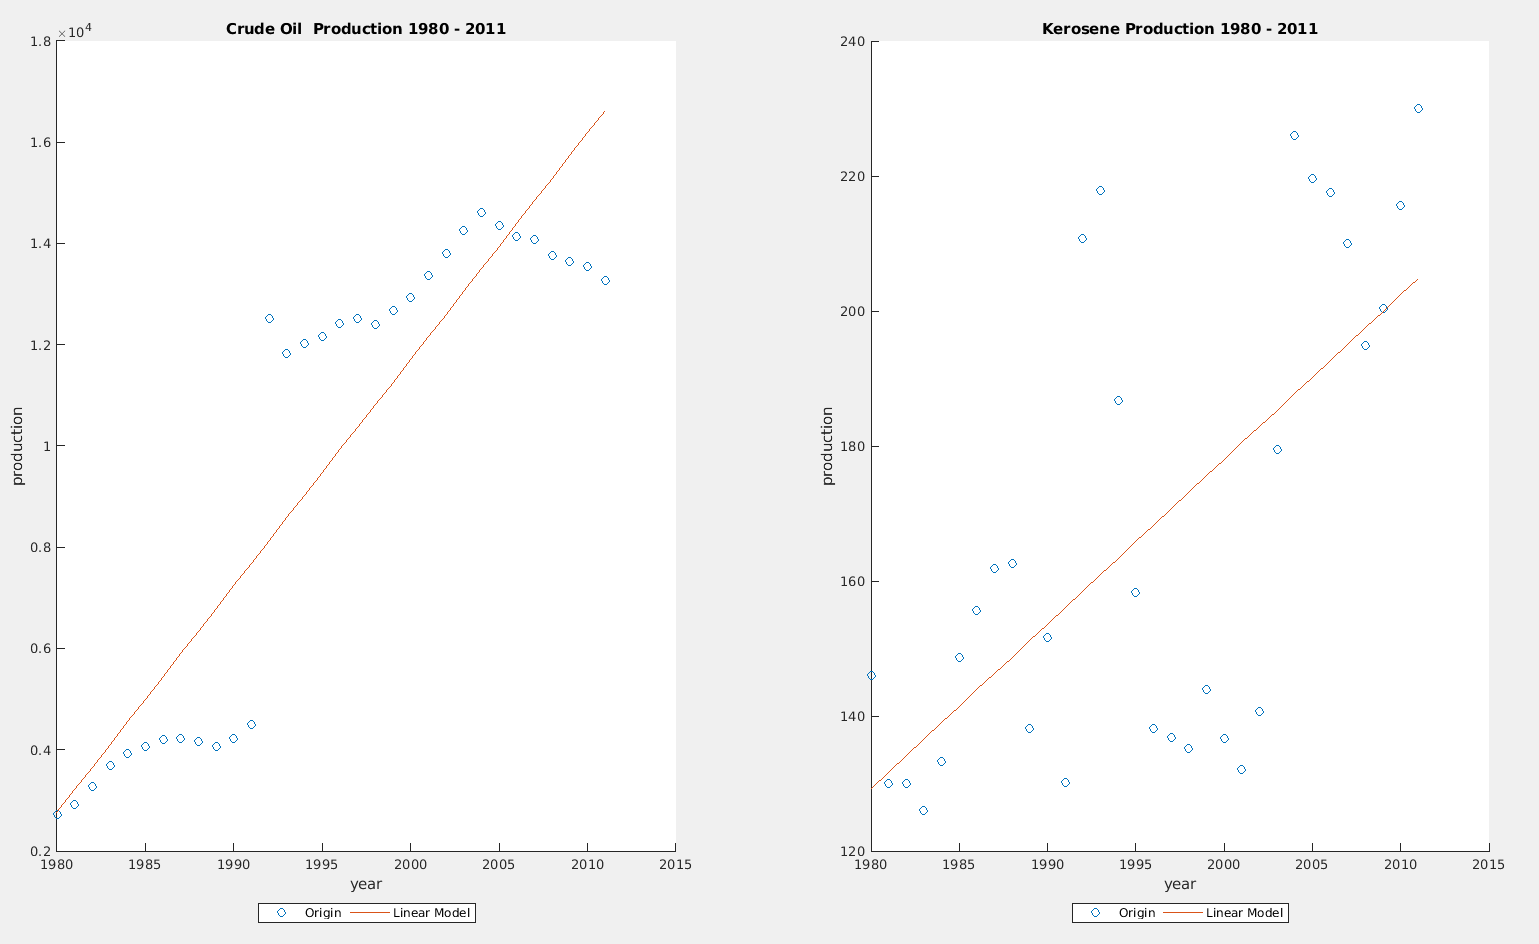
\includegraphics[width=0.9\linewidth]{./figures/ex2b.png}
    \end{minipage}
  \caption{Linear Model and original data of crude oil and kerosene production from 1980 to 2011}
\end{figure}
\vspace{20px}
\item Consider the quadratic model ${y_i = \alpha_1 + \alpha_2x_i + \alpha_3x^2_i}$ and apply it to the crude oil and kerosene production
data in the period 1980-2011. Write a script \textit{quadraticModel.m} in which you use \textit{leastSquares()} to
compute the least squares solution ${x^*}$ and the metrics of the residual. For each dataset, create a figure in which
you plot the original data points and the quadratic model.

The general flow of the logic is very similar, but the matrix A is extended via the same logic so it would produce bigger least square vector (there are 3 columns now). Then instead of ${y_i = mx_i + b}$, quadratic modelling equation ${y_i = a + bx_i + cx_i^2}$ is used. \\
\vspace{20px}
 \begin{lstlisting}[language=Matlab]
    same as before ...
    x = [ones(duration, 1), year(:), year(:).^2];

    [factors, ~, ~, ~] = leastSquares(x, y);

    z = factors(1) + factors(2) * year(:) + factors(3) * year(:).^2;
    same as before ...
 \end{lstlisting}
 As a result of that change, resulting graph (quadratic) became more fitting than the previous linear graph shown in figure 1.
 \vspace{20px}
 \begin{figure}[h!]
    \begin{minipage}[c]{1\linewidth}
        \centering
        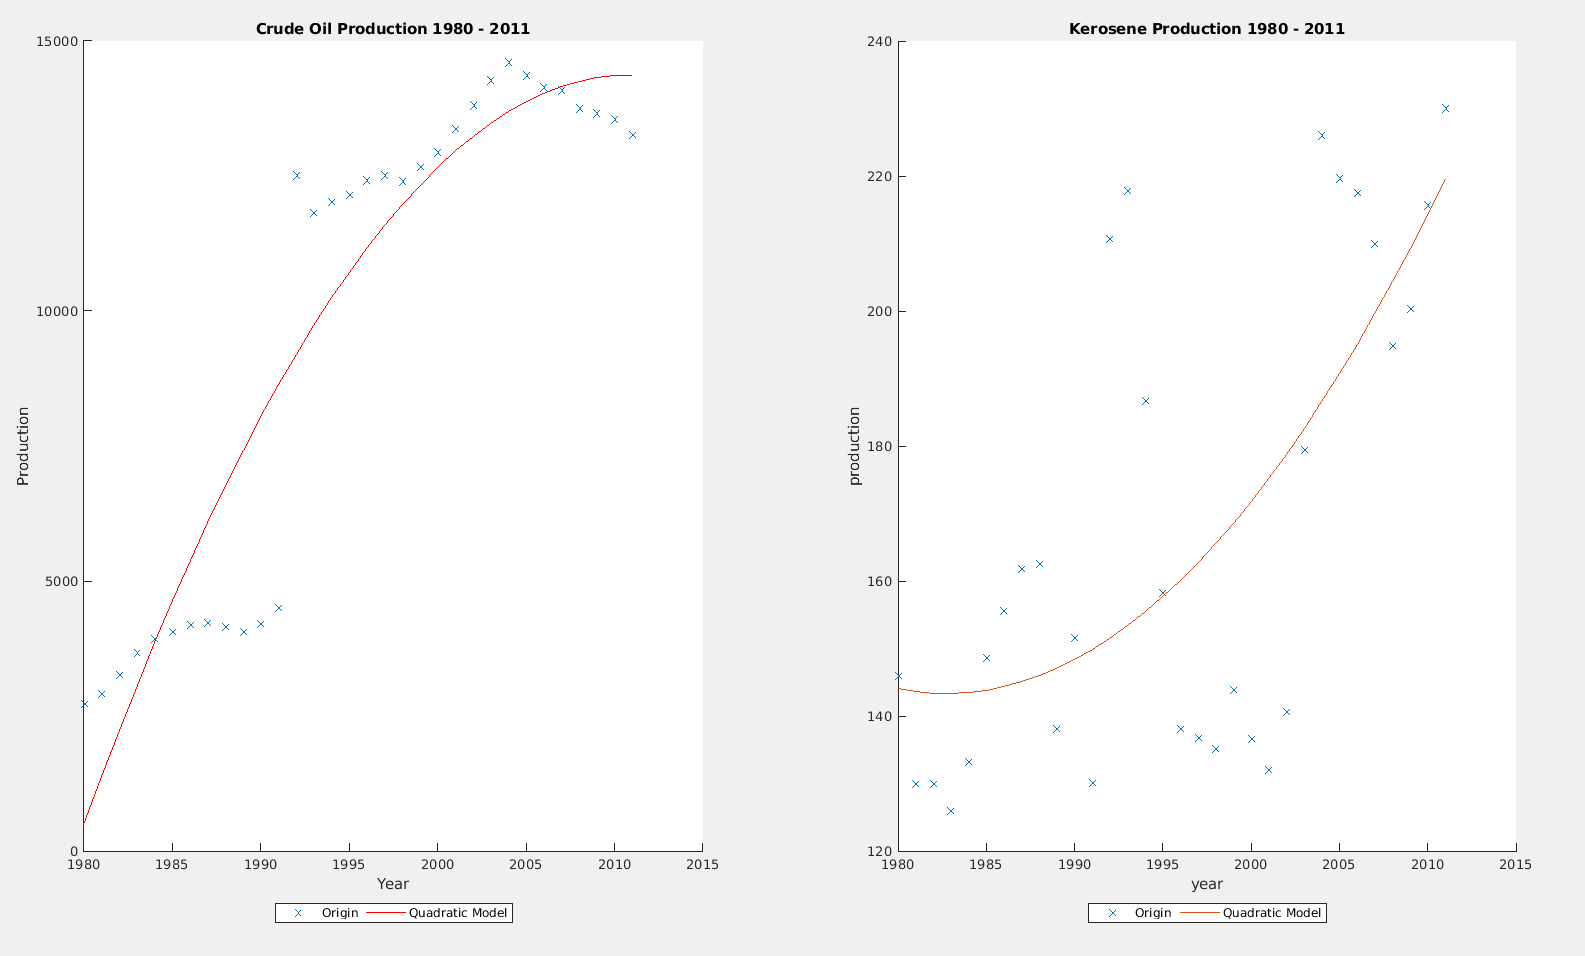
\includegraphics[width=0.9\linewidth]{./figures/ex2c.png}
    \end{minipage}
  \caption{Quadratic Model and original data of crude oil and kerosene production from 1980 to 2011}
\end{figure}

\item Consider the cubic model ${y_i = \alpha_1 + \alpha_2 x_i + \alpha_3 x^2_i + \alpha_4 x^3_i}$ and apply it to the crude oil and kerosene production
data in the period 1980-2011. Write a script \textit{cubicModel.m} in which you use \textit{leastSquares()} to com-
pute the least squares solution ${x^*}$ and the metrics of the residual. For each dataset, create a figure in which you
plot the original data points and the cubic model.

We can apply the same approach as ${(c)}$ and just increase the size of least squares vector and change the slope calculation from ${y_i = a + bx_i + cx_i^2}$, to ${y_i = a + bx_i + cx_i^2 + dx_i^3}$

\newpage

Code can be altered as following: \\

\begin{lstlisting}[language=Matlab]
    x = [ones(duration, 1), year(1:duration), 
                            year(1:duration).^2, 
                            year(1:duration).^3];

    [factors, ~, ~, ~] = leastSquares(x, y(1:duration));

    z = factors(1) + factors(2) * year(1:duration)
                + factors(3) * year(1:duration).^2 
                + factors(4) * year(1:duration).^3;

\end{lstlisting}

Finally, the resultant graph would be more fitted to the original data points than other approaches. Especially for the crude oil production.\\

 \vspace{20px}
 \begin{figure}[h!]
    \begin{minipage}[c]{1\linewidth}
        \centering
        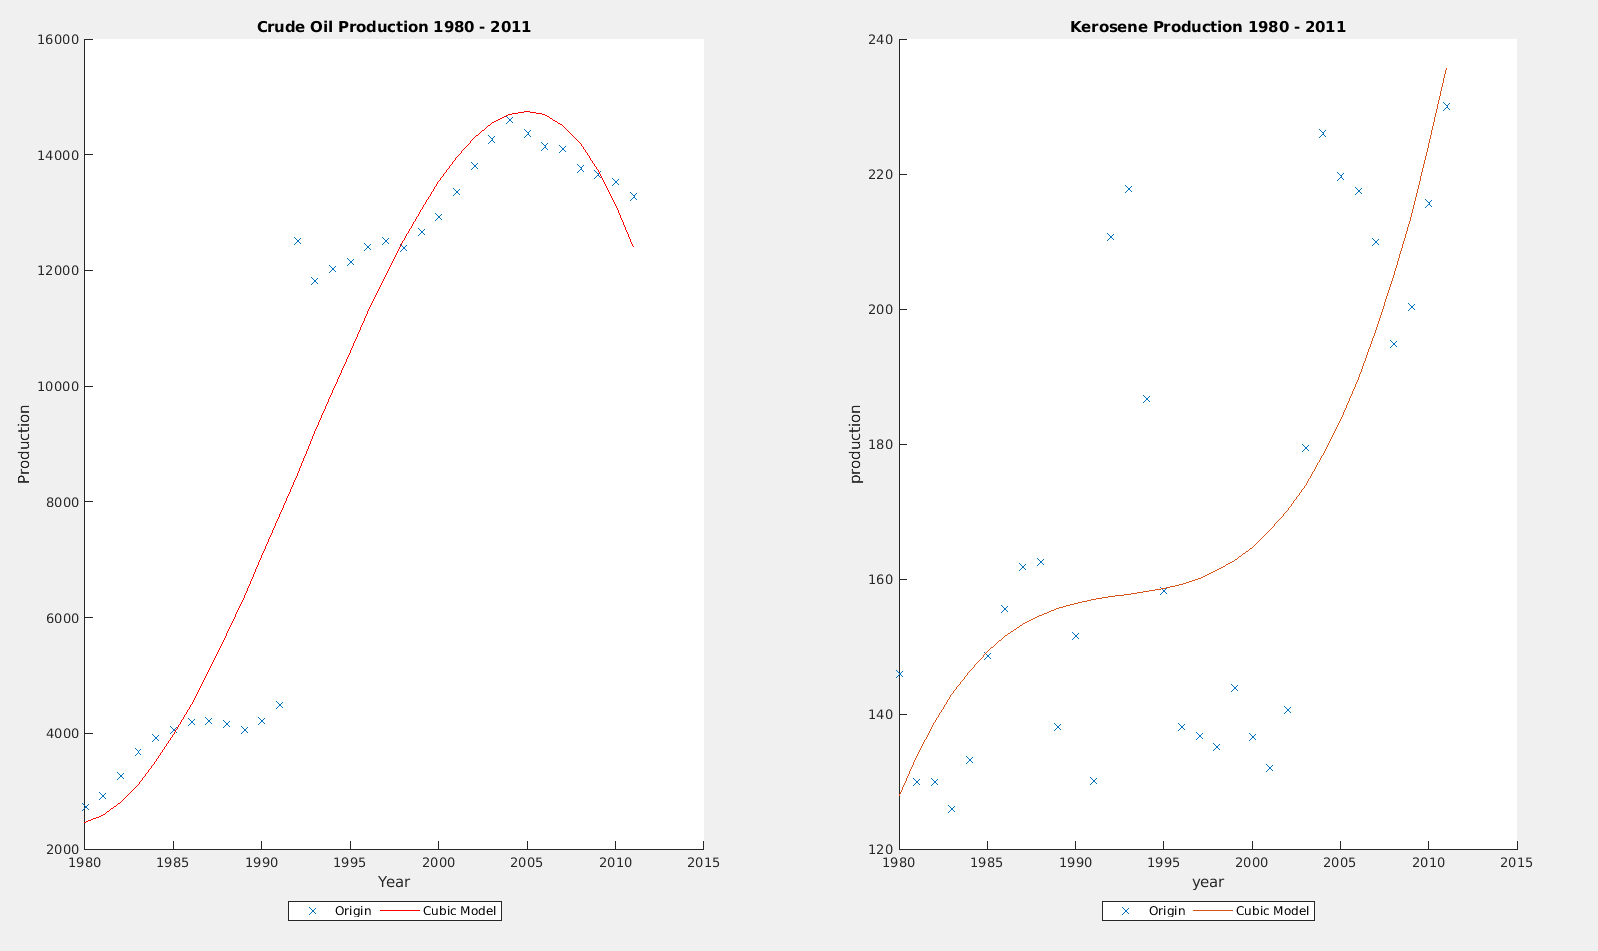
\includegraphics[width=0.9\linewidth]{./figures/ex2d.png}
    \end{minipage}
  \caption{Cubic Model and original data of crude oil and kerosene production from 1980 to 2011}
\end{figure}
\vspace{20px}

\item Compare the linear, quadratic and cubic models on the basis of the quality metrics computed above, by creating
a table containing the results for the two models. Which one of the three models would you pick for the crude
oil data? And for the kerosene? Provide an estimate of the crude oil and kerosene production in 2012 by using
the three models and compare the values obtained with the real values reported in the data source. Comment on
your results. \\

\newpage

\begin{center}
\begin{tabular}{|l|r|r|r|r|} \hline
Model Type & EuclideanNorm & Standard Error & RMSE \\
\hline
  Linear Crude  & 11,471 & 131,590,000 & 2,027.8\\
\hline
  Quadratic Crude & 9,582.6 & 91,827,000 & 1,694\\
\hline
  Cubic Crude & 7,917.9 & 62,692,000 & 1,399.7 \\
  \hline
  Linear Kerosene & 151.0222 & 22,808 & 26.6972\\
\hline
  Quadratic Kerosene & 145.3013 & 21,112 & 25.6859\\
\hline
  Cubic Kerosene & 138.476 & 19,175 & 24.4793 \\
  \hline
\end{tabular}
\end{center}

\vspace{20px}

\begin{tabular}{|l|r|r|r|r|} \hline
Energy Type & Linear Estimation & Quadratic Estimation & Cubic Estimation & Real Data \\
\hline
 Crude Oil & 17,082(30.3\%) & 14,344(+9.4\%) & 11,473 (-12.5\%) & 13,111\\
\hline
Kerosene & 207.2856(-23.6\%) & 225.1621 (-16.9\%) & 248.4740 (-7.3\%) & 267.89\\
\hline
\end{tabular}
\vspace{20px}

To make a simple analysis, having a smaller Euclidean Norm suggests better fit of the model to the original data as smaller euclidean norm indicates smaller residuals, and naturally bigger would indicate the opposite. Similarly, Standard Error (SE) and Root Mean Squared Error (RMSE) indicates better fit of the model when they are small. \\

Under this assumption, the data on the table suggests for all the cases, cubic model is the best, quadratic model is the second, and linear model is the worst model to fit the original data. \\

However, the prediction made for 2012 from these models suggest, even though cubic model proved to be the best for kerosene production trend prediction, in terms of prediction for crude oil production, quadratic model showed more accurate result. However, prediction of a singular value is not enough to make a conclusion that quadratic model will always perform better for kerosene production prediction or cubic model will always perform better for crude oil production prediction as the 2012 data might have been just a singular anormaly in the data.\\

To get a more concrete conclusion, we would need more historical data and also make more predictions based on the obtained model. However, statistically it is undeniable that cubic model will show the best predictions.\\

\end{enumerate}
\vspace{20px}

\newpage
\section*{Exercise 3: Analysis of periodic data [20 points]}

The file \textit{temperature.txt} contains the area mean-temperatures of Switzerland between January 1864 and March
2021 included. Temperature data exhibit a periodic behaviour and we will try to capture it by using periodic models.
You will need the function \textit{leastSquares()} implemented in Exercise 2. \\

\begin{enumerate}[label=(\alph*)]
 \item Consider the periodic model ${y_i = \alpha_1 + \alpha_2 cos(2\pi x_i ) + \alpha_3 sin(2\pi x_i )}$ and apply it to the temperature data:
(I) between January 1960 and January 1963; (II) between January 1960 and January 1970. Write a script
\textit{periodicA.m} in which you compute the least squares solutions and the metrics of the residual, and plot the
outputs of the model against the original data in both cases. \\

\begin{lstlisting}[language=Matlab]
    [x1, y1] = readTemperatureData(filepath, startYear, endYear);
    x = [ones(length(x1), 1), cos(2 * pi * x1), sin(2 * pi * x1)];
    [factors, ~, ~, ~] = leastSquares(x, y1);
    h = height(x1);

    z = factors(1) + 
        factors(2) * cos(2 * pi * x1(1:h)) + 
        factors(3) * sin(2 * pi * x1(1:h));
    generate graphs...
\end{lstlisting}

The ${temperature.txt}$ file is read in a bit of a different way as the structure of the data is different. It can be seen in ${readTenoeratureData.m}$ file. Then the x-axis data is converted into the periodic model format given in the question. Then the residual vector is calculated using ${leastSquares.m}$ which was completed in the previous question. Then periodic model graph is calculated and graphed along with original data points. The resulting graph is as following: \\

 \begin{figure}[h!]
    \begin{minipage}[c]{1\linewidth}
        \centering
        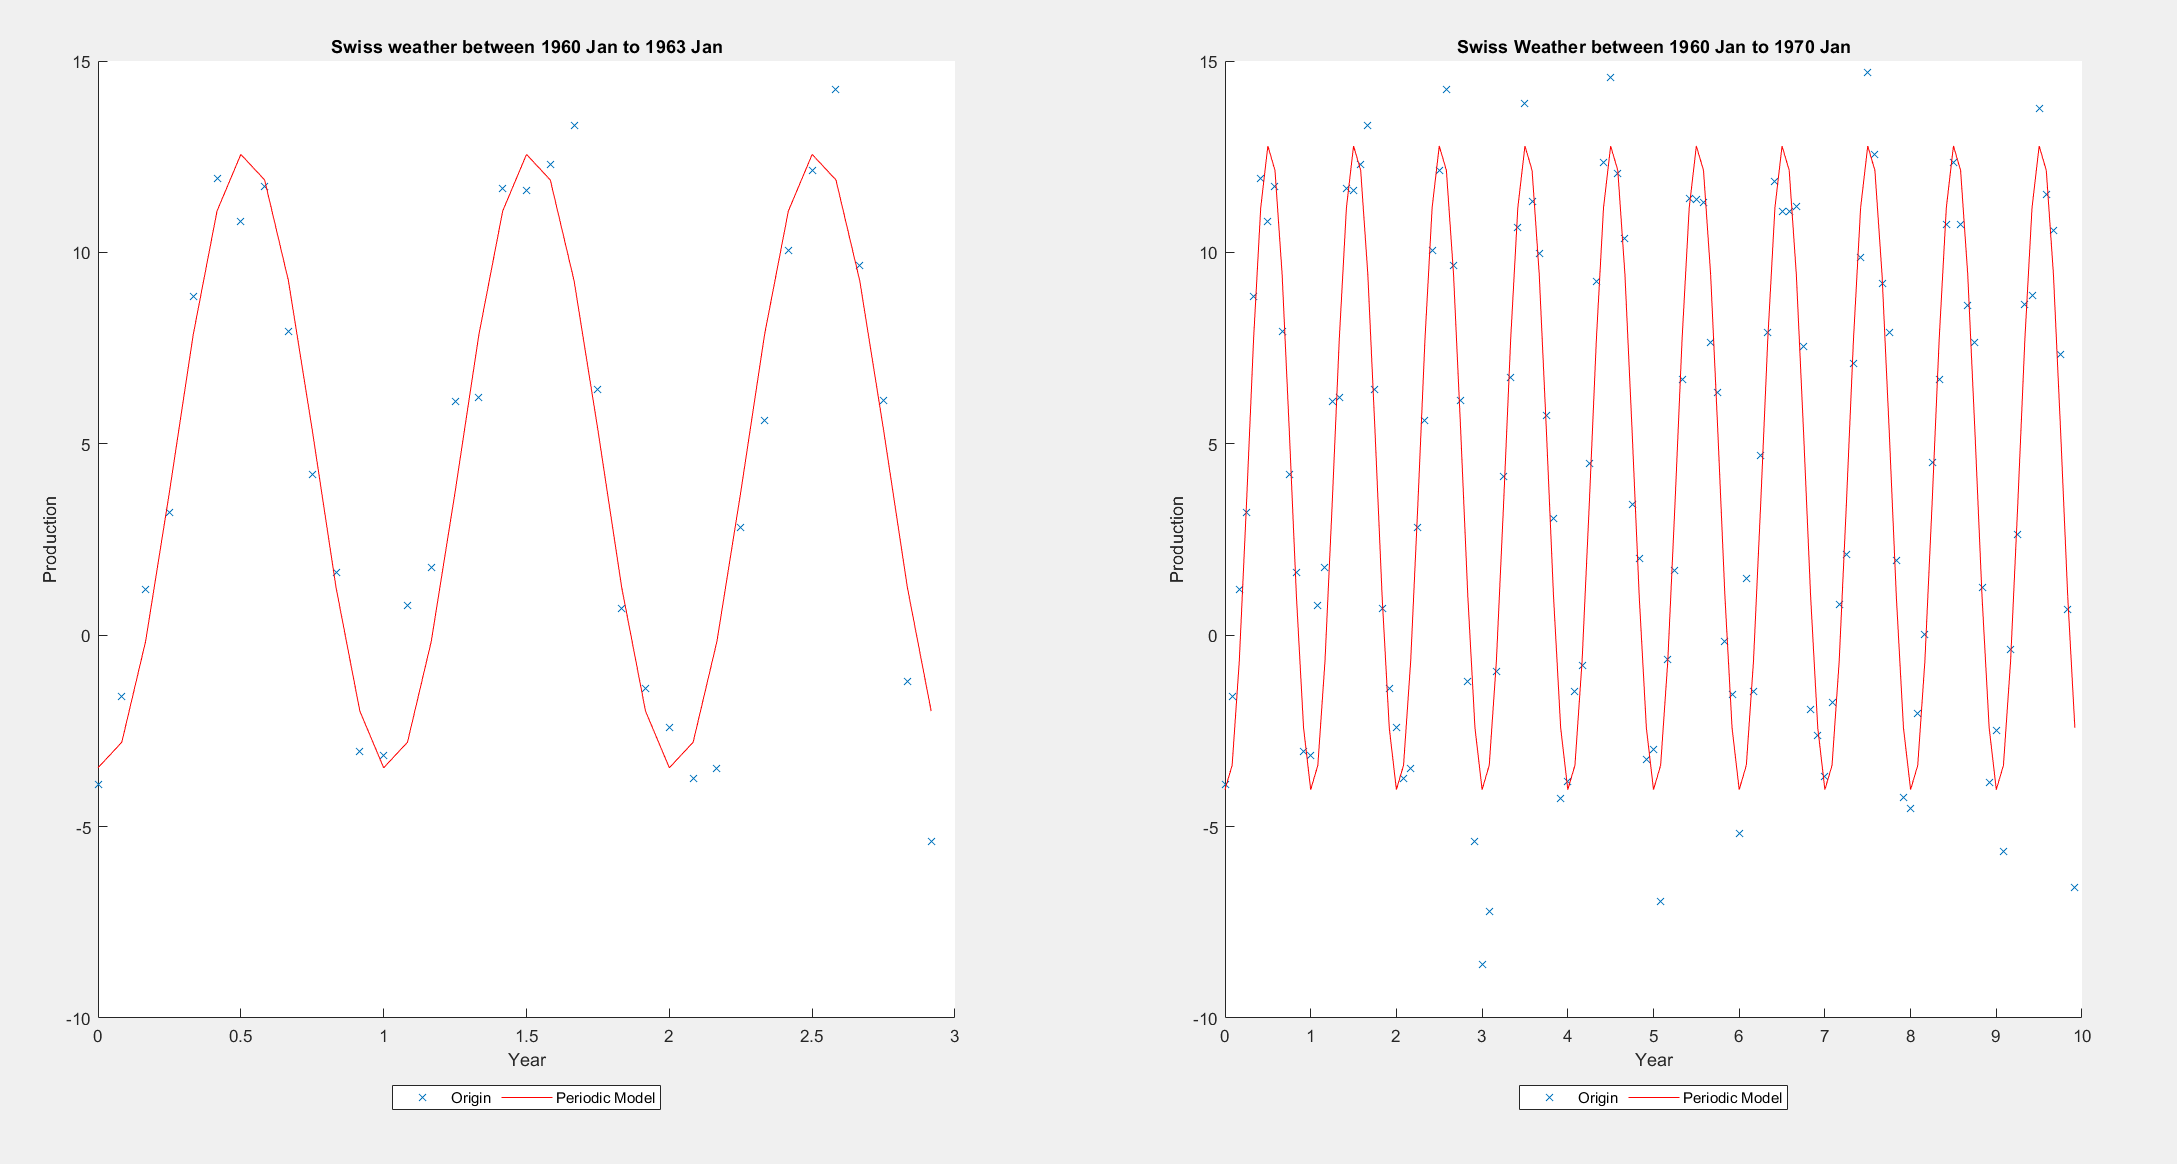
\includegraphics[width=0.9\linewidth]{./figures/ex3a.png}
    \end{minipage}
  \caption{Periodic model of swiss weather 1960 Jan to 1963 Jan (left) and 1960 Jan to 1970 Jan (right)}
\end{figure}

\newpage

\item Repeat the same analysis and plots of the previous point for both time series, by using the periodic model
${y_i = \alpha_1 + \alpha_2 cos(2\pi x_i ) + \alpha_3 sin(2\pi x_i ) + \alpha_4 cos(4\pi x_i)}$ in the script \textit{periodicB.m}.

Only things that need to be added are as following:

\begin{lstlisting}[language=Matlab]
    ...
    x = [ones(length(x1), 1), cos(2 * pi * x1), 
         sin(2 * pi * x1), cos(4 * pi * x1)];
    ...
    z = factors(1) + 
        factors(2) * cos(2 * pi * x1(1:h)) + 
        factors(3) * sin(2 * pi * x1(1:h)) +
        factors(4) * cos(4 * pi * x1(1:h));
    ...
\end{lstlisting}

Resulting graph is as following: \\

 \begin{figure}[h!]
    \begin{minipage}[c]{1\linewidth}
        \centering
        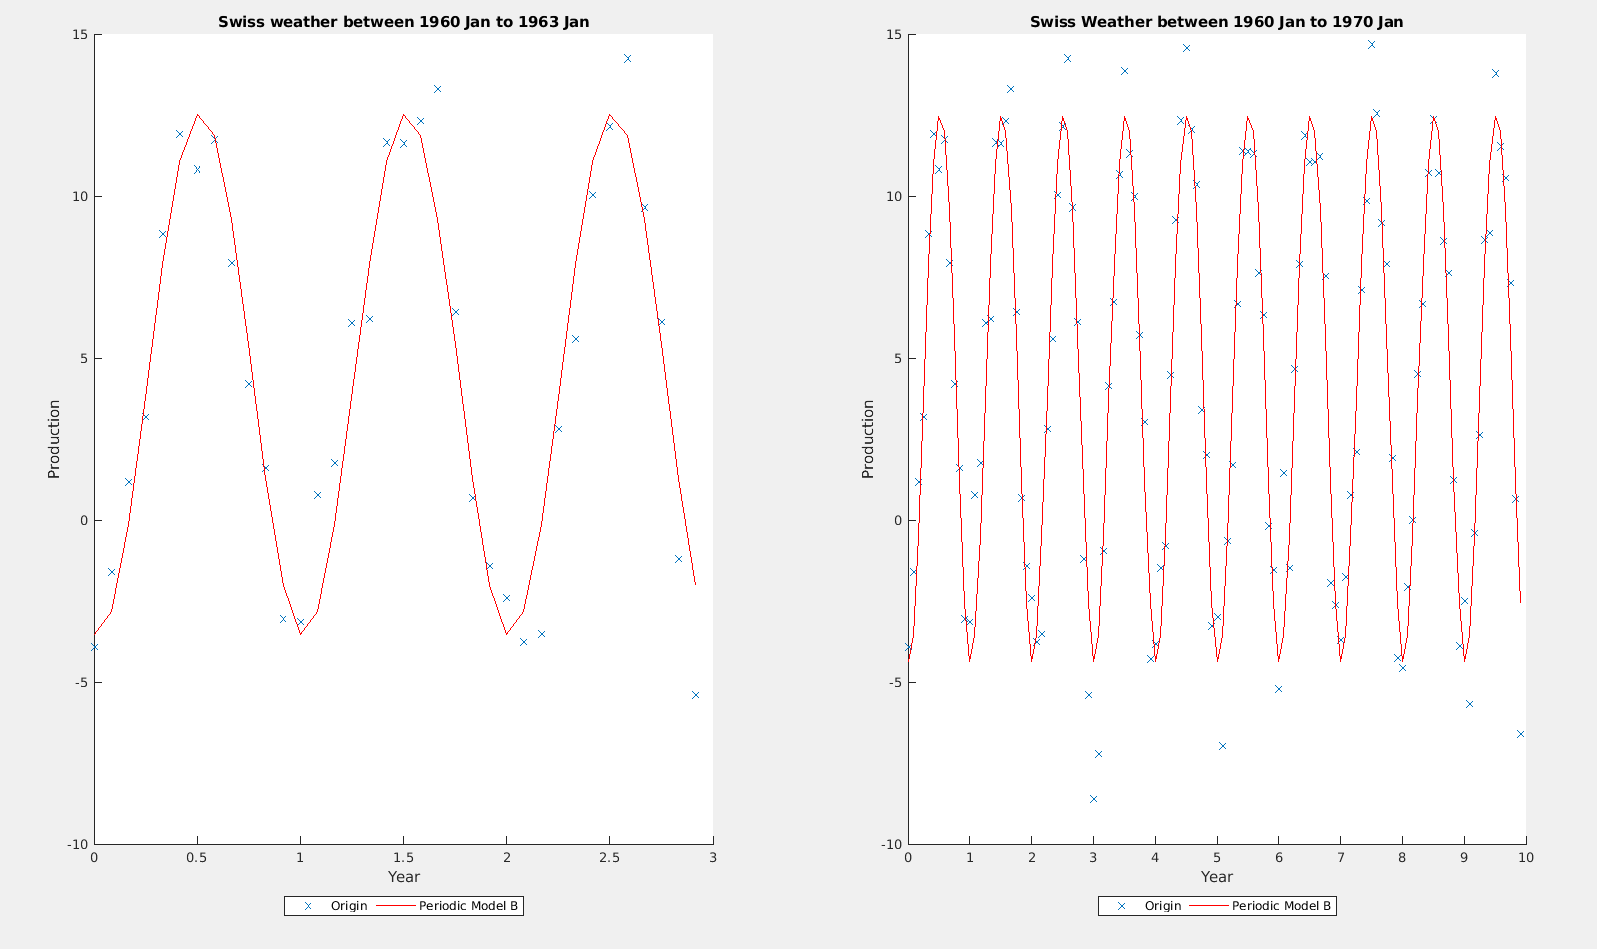
\includegraphics[width=0.9\linewidth]{./figures/ex3b.png}
    \end{minipage}
  \caption{Periodic model 'B' of swiss weather 1960 Jan to 1963 Jan (left) and 1960 Jan to 1970 Jan (right)}
\end{figure}

\vspace{10px}

\item Compare the models of point ${(a)}$ and ${(b)}$. Was it beneficial to include more data? Which model would you
prefer? Are you satisfied with the results obtained? If necessary, what would you suggest to improve your
models? Motivate your answers. \\

\begin{center}
\begin{tabular}{|l|r|r|r|r|} \hline
Model Type & EuclideanNorm & Standard Error & RMSE \\
\hline
  Periodic A short  & 10.0838 & 101.6826 & 1.6806\\
\hline
  Periodic A long & 18.0011 & 324.0413 & 1.6433\\
\hline
  Periodic B short  & 10.0807 & 101.6201 & 1.6801\\
\hline
  Periodic B long & 17.8216 & 317.6092 & 1.6269\\
\hline
\end{tabular}
\end{center}

\vspace{20px}

From the graph generated alone, it becomes very obvious that there is barely any difference between the two models. The negligence of 2 model's difference becomes more apprent through the display of quality metrics through a table. Naturally, the necessity to add more data becomes also negligible and almost pointless. Hence, periodic model A will be more preferable as it would be easier to calculate with lower time complexity due to smaller input and residual vector resulting from it. \\

Generally, it seems like periodic models are fitting the original datapoints quite well. However, if there has  To make an improvement to it, maybe values other than ${2\pi}$ can be used with more data to increase accuracy, for example, ${\pi}$.

\end{enumerate}

\section*{Exercise 4: Data linearization and Levenberg-Marquardt method for the exponential model [20 points]}
\vspace{20px}
The file \textit{nuclear.txt} contains the data on the nuclear electric power consumption by year in China in the period
1999-2006. We consider the power law model, expressed as: \\

\begin{equation}
y_i = \alpha_ix_i^{\alpha_2}
\end{equation}

\vspace{20px}

\begin{enumerate}[label=(\alph*)]
 \item Find the least squares best fit by using data linearization and compute the RMSE both of the log-linearized
model and of the original exponential model. Include in your report all the computations and the necessary
steps, as explained in the slides of the tutorial. \\

Log-Linearization can be done using the power law model shown in the beginning of the question. To convert it into linear function, ${ln()}$ can be applied to both of the sides, then due to the properties of logarithms, the power law model can be expressed as following: \\

\begin{equation}
 ln(y_i) = ln(\alpha_1) + \alpha_2 ln(x_i)
\end{equation}

For original exponential model, it can be expressed as the following: \\

\begin{equation}
 y_i = \alpha_ie^{\alpha_2x_i}
\end{equation}

Which then can be converted applying ${ln()}$ to both sides again and get the following linear expression: \\

\begin{equation}
 ln(y_i) = ln(\alpha_1) + \alpha_2x_i
\end{equation}

Equation 8 and 10 can be used to build the original exponential model and the log-linearization model using the previously defined ${leastSquare}$ function. Important factor to remember during the implementation would be that the calculated result of the model would be equivalent to ${ln(y_i)}$ not the ${y_i}$, hence, the result would have to be used as the power of ${e}$ and not be graphed directly in relation to the original data. \\

\newpage

\begin{lstlisting}[language=Matlab]
    % Getting x = year and y = consumption data.
    [year, consumption, change] = readData('../data/nuclear.txt');
    
    % Manipulate x-vals so it starts from 1
    xaxis = year - min(year) + 1;
    % Convert x and y values into log forms
    logX = log(xaxis);
    logY = log(consumption);
    
    h = height(logX);
    
    % Create a coefficient matrix with 1s and log form of x values to  
    % pas it onto the leastSquare calculation to get 2d residual 
    % vector (alphas) according to eq8
    X = [ones(h, 1), logX];
    
    % Call least square function with predefined matrix and log form of Y
    % to obtain residual vectors (factors) and RMSE for this model
    [factors, ~, ~, rmse_log] = leastSquares(X, logY);
    
    % Calculate the log-linearization model fitting the given data
    % We are taking the logX as multiplicand, the same form as the 
    % coefficient passed for leastSquares function
    % the result is powered by 'e' because the result without it will
    % be equivalent to 'y' values used in least square function
    % which were logged.
    z = exp(factors(1) + factors(2) * logX);
    
    ... print the residual vector and the rmse of the model ...
    
    % Just in case, re-calculate the log for of the y-axis
    logYO = log(consumption);

    hO = height(xaxis);
    
    % Create a coefficient matrix with 1s and x-axis values
    % to get 2d residual vector (alphas) for original exponential model
    XO = [ones(hO, 1), xaxis];
    
    % Calculate the residual vector (factorsO) and RMSE value
    % (rmse_original)
    % of the original exponential method through leastSquares function
    [factorsO, ~, ~, rmse_original] = leastSquares(XO, logYO);
    
    % Calculate original exponential model values fitting to this data
    % exp() function called for same reason as calculation of 'z'
    zO = exp(factorsO(1) + factorsO(2) * xaxis);
    
    ... print the residual vector and the rmse of the model ...
\end{lstlisting}

The full script can be viewed at ${ex4b.m}$ in \textit{src} folder. 

\begin{center}
\begin{tabular}{|l|r|r|} \hline
  & Original Exponential Model & Log-Linearization Model \\
\hline
  RMSE & 5.4672  & 5.0953 \\
\hline
  ${\alpha_1}$ & 2.3554 & 2.3705 \\
\hline
  ${\alpha_2}$ & 0.2257 & 0.7549 \\
\hline
\end{tabular}
\end{center}

 \begin{figure}[h!]
    \begin{minipage}[c]{1\linewidth}
        \centering
        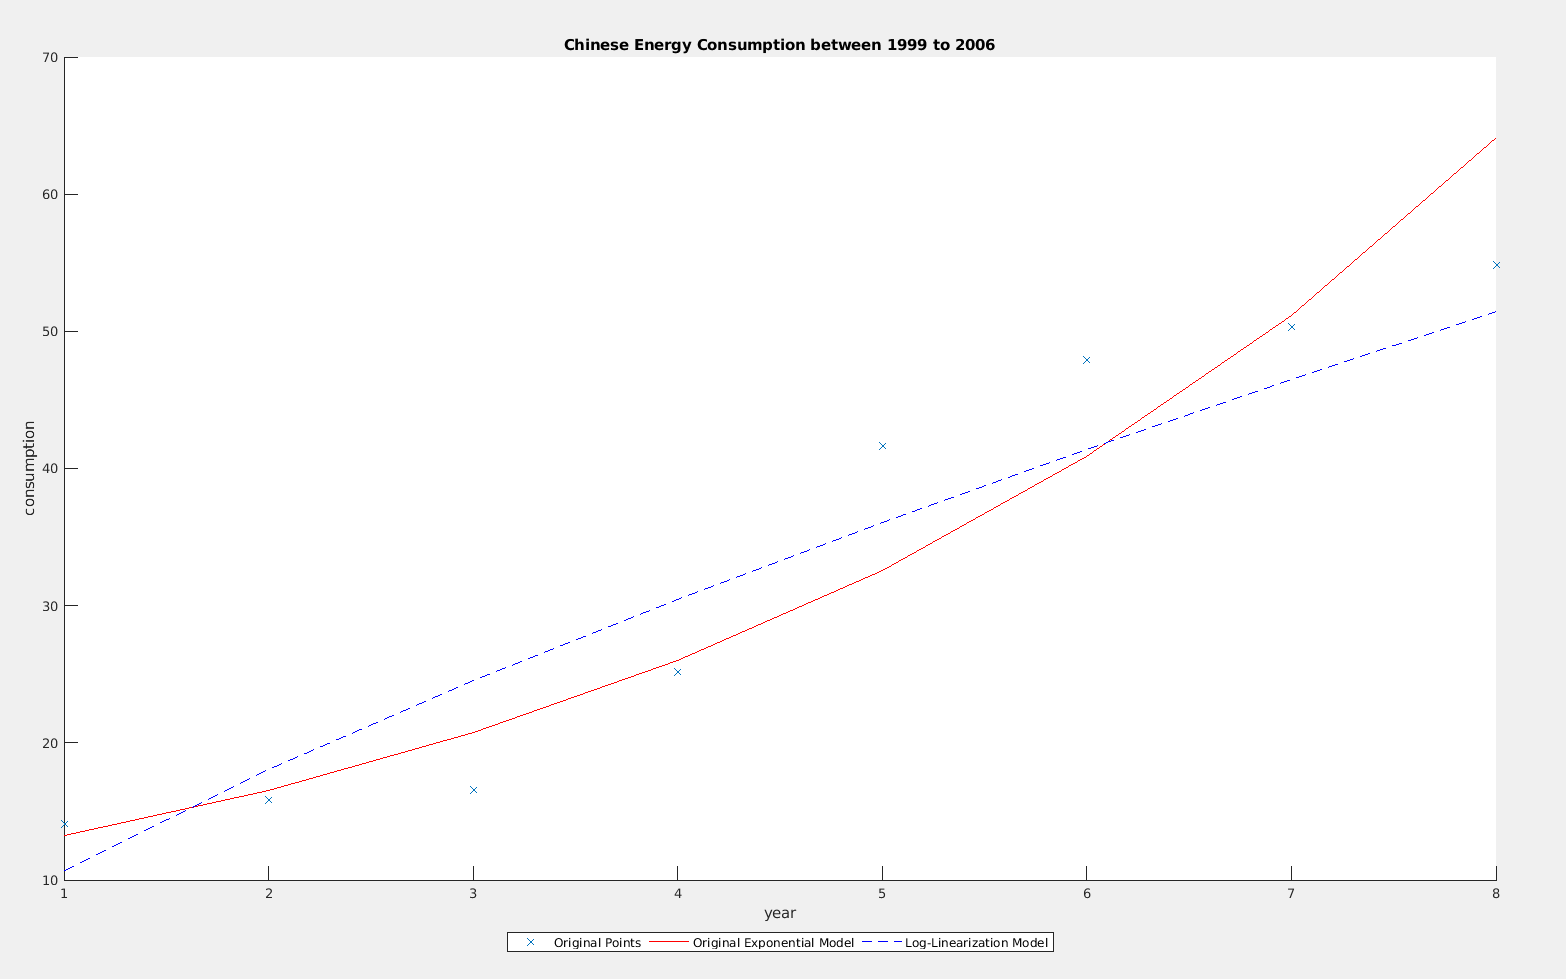
\includegraphics[width=0.9\linewidth]{./figures/ex4a.png}
    \end{minipage}
  \caption{Original exponential model and Log-linearization model with original data of Chinese electricity consumption between 1999 to 2006}
\end{figure}

\vspace{20px}

\item Write a function \textit{levenbergMarquardt()} in which you implement the Levenberg-Marquardt algorithm for
solving nonlinear least squares problems. Following again the slides of the tutorial, show how you can formulate
the problem in order to solve it with Levenberg-Marquardt method and compute analytically all the necessary
quantities. Finally, write a script \textit{ex4b.m} in which you use the function \textit{levenbergMarquardt()} to fit
the data points and compute the RMSE. \\

Logic behind the Levenberg Marquardt algorithm is an alteration on Gauss-Newton method using ${\lambda}$ (Gaussian-Newton method is equivalent to Levenberg Marquardt algorithm when ${\lambda = 0}$). The difference is that this algorithm tackles eventual ill-conditioning of Jacobian matrix by introducing a regularization. \\

\begin{lstlisting}
Given a random initial guess x^0 and lambda
    for i = 0, 1, 2, . . . do
        A = Jr(x(i))
        v(i) = (-1) * (A^T * A + lambda * diag(A^T * A))^(-1)
                * A^T * r(x(i))
        x(i+1) = x(i) + v(i)
        if (norm(v(i)) < tolerance) {
            return 1; // exit with success
        }
    end for
    return 0; exit with failure
\end{lstlisting}

Important aspect of implementing this algorithm is the definition of Jacobian matrix and calculation of residuals ${(r(x_i))}$. Jacobian matrix can be expressed as following for the power law model which is our basis equation: \\

\begin{equation}
 J_r(\alpha_1, \alpha_2) = \begin{bmatrix}
            x_1^{\alpha_2} & \alpha_1x_1^{\alpha_2}log(x_1) \\
            ... & ... \\
            x_i^{\alpha_2} & \alpha_1x_i^{\alpha_2}log(x_i) \\
       \end{bmatrix}
\end{equation}

\vspace{20px}

Residual calculation can be expressed as following for the power law model: \\

\begin{equation}
 r(\alpha_1, \alpha_2) = \begin{bmatrix}
            \alpha_1 x_1^{\alpha_2} - y_1\\
            ... \\
            \alpha_1 x_i^{\alpha_2} - y_i\\
       \end{bmatrix}
\end{equation}

With these factors in mind, the \textit{levenbergMarquardt()} is implemented in \textit{levenbergMarquardt.m} script and resultant graph is plotted with other least squares best fit model graphs. The result is as following: \\

 \begin{figure}[h!]
    \begin{minipage}[c]{1\linewidth}
        \centering
        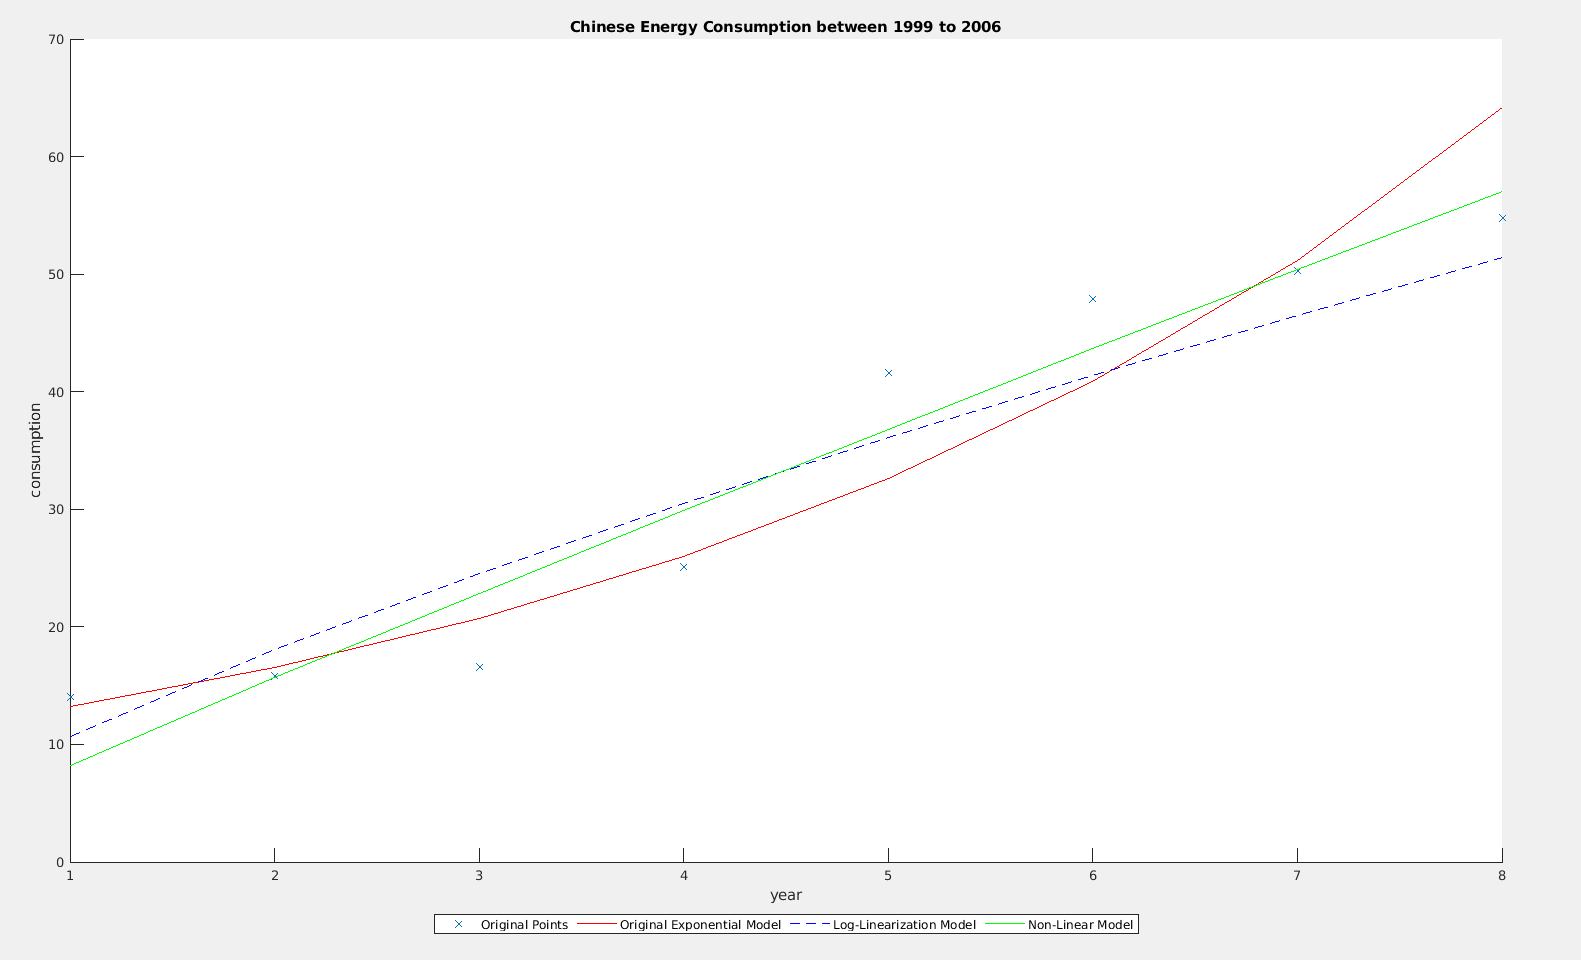
\includegraphics[width=0.9\linewidth]{./figures/ex4b.png}
    \end{minipage}
  \caption{Original exponential model and Log-linearization model and non-linear model with original data of Chinese electricity consumption between 1999 to 2006}
\end{figure}

View the ${ex4b.m}$ to see the implementation of the models. \\

\newpage

\item Compare the results obtained in points (a) and (b), by extending the script ${ex4b.m}$ to produce a plot of the
original data points together with the two models. Which model would you choose? \\

The root mean square error (RMSE) for Original Exponential Model and Log-Linearization Model were calculated before which were 5.4672 and 5.0953. Newly calculated RMSE for Non-Linear Model using Levenberg Marquardt is 4.2394. Like explained before, lower RMSE indicates better fit, hence, out of 3 models Non-Linear Model has the best fit to the original data points. Which was also obvious through the graph in figure 7 itself. Naturally, it would be the wisest to choose Non-Linear Model to predict the data in this scenario.

\end{enumerate}


\section*{Exercise 5: Tikhonov regularization [15 points]}
Given the ill-posed problem ${Ax = b}$, with ${A \in R^{n\times m}}$ and ${b \in R^m}$, we aim to solve it using linear
least squares with Tikhonov regularization, which is formulated as

\begin{equation}
 min_x \norm{Ax - b}^2 + \alpha \norm{x}^2
\end{equation}

where ${\alpha \in R}$ is a regularization parameter.

\begin{enumerate}[label=(\alph*)]
 \item Derive analytically the optimal solution ${x^*}$ of equation13. What is the purpose of the parameter 
 ${\alpha}$ and how should
we proceed to choose its value?
\end{enumerate}



\end{document}
